\section{Rule generation} \label{sec: rule gen}
After the investigation of minimum support as well as different metrics for rule generation, we remove attributes such as \verb|surgery|, \verb|site of lesion|, \verb|outcome| and \verb|hospital number|. This removes some bias from the data, and allows for more exploratory learning. In this section, \verb|abdomen| is chosen as the class attribute for classification with association rule analysis.

\begin{figure}[H]
\centering
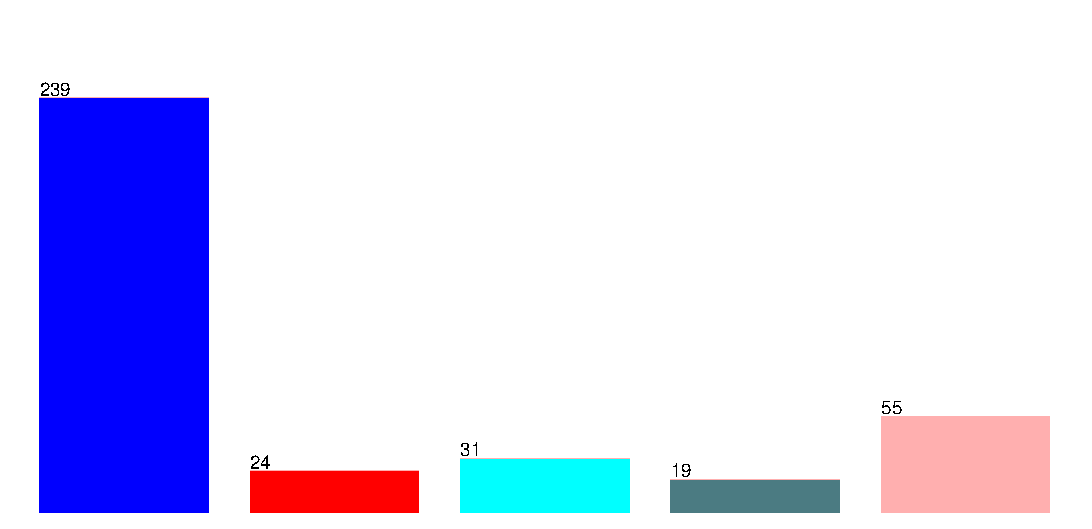
\includegraphics[scale=0.8]{abdomen-class}
\caption{Distribution of the \textit{abdomen}-attribute, with values: distended lg intestine, other, Normal, Firm feces in the lg intestine, Distended small intestine}
\end{figure}

\begin{verbatim}
	weka.associations.Apriori -R -N 1000 -T 0 -C 0.4 -D 0.05 -U 0.42 -M 0.1 -S -1.0 -A -c 20
\end{verbatim}
\begin{itemize}
\item \verb|231. pain=Continous severe|

\verb|pain peristalsis=Absent |

\verb|rectal examination - feces=Decreased |

\verb|abdominocentesis appearance=Cloudy 46|
 
\verb| ==> |

\verb|abdomen=Distended lg intestine 44   |

\verb|conf:(0.96)|
\end{itemize}
\begin{verbatim}
	weka.associations.Apriori -R -N 1000 -T 0 -C 0.95 -D 0.05 -U 0.42 -M 0.1 -S -1.0 -c 20
\end{verbatim}
\begin{itemize}
\item \verb|1. pain=Continous severe pain|

\verb|nasogastric reflux=>1liter |

\verb|abdominocentesis appearance=Cloudy 55|

 \verb| ==> |
 
 \verb|abdomen=Distended lg intestine 55 |

 \verb| <conf:(1)> lift:(1.54) lev:(0.05) [19] conv:(19.28)|
\end{itemize}

\begin{verbatim}
	weka.associations.Apriori -R -N 1000 -T 1 -C 4.0 -D 0.05 -U 0.42 -M 0.1 -S 0.01 -c 20
\end{verbatim}

\begin{itemize}
\item  \verb|21. temperature of extremities=Cool|

\verb|peripheral pulse=Reduced |

\verb|pain=Continous severe pain|

\verb|nasogastric tube=None |

\verb|abdominocentesis appearance=Cloudy 41 |

\verb|==> |

\verb|peristalsis=Absent |

\verb|abdominal distension=Severe |

\verb|abdomen=Distended lg intestine 37    |

\verb|conf:(0.9) < lift:(4.55)> lev:(0.08) [28] conv:(6.57)|
\end{itemize}
